% !TeX root = 11gy_cpp
\documentclass[../cpp_book/cpp_book.tex]{subfiles}
\begin{document}
	\onlyinsubfile{
		\begin{center}
			{\LARGE\textbf{C++}}
			
			{\Large Gyakorlat jegyzet}
			
			2 óra.
		\end{center}
		A jegyzetet \textsc{Umann} Kristóf készítette \textsc{Horváth} Gábor gyakorlata alapján. (\today)
	} 
	\section{Objektum orientált programozás}
	Manapság az egyik legnépszerűbb programozási paradigma a objektum orientált programozás (\textit{object oriented programming}, röviden \textit{OOP}). Bár sokféleképpen definiálhatjuk, e három dolgot azonban általában megköveteljük egy objektum orientált kódtól:
	\begin{compactitem}
		\item enkapszuláció, azaz az adatok egybefoglalása
		\item kód újrafelhasználás
		\item adat elrejtés
		%TODO elmagyarázni ezeket
	\end{compactitem}
	Fontos, hogy az objektum orientáltságot ne kössük feltétlenül az osztályokhoz, ezeket a követelményeket ugyanis ha körülményesen is, de nélkülük is meg tudjuk oldani. Példaképp, C-ben létrehozhatunk egy egyszerű rekordot, melynek deklarációját és a hozzá tartozó műveleteket eltároljuk egy header fájlban, magát a rekordot és a függvényeket csak egy fordítási egységben definiáljuk. Ezzel elértük az enkapszulációt, az adatok rejtve vannak, és egy ilyen rekordot el tudunk tárolni egy másik rekordban is könnyedén, ezzel megvalósítva a kód újrafelhasználást.

	Így bátran kijelenthetjük, hogy a C nyelv egy olyan nyelv, mely támogatja az objektum orientált programozást. Azonban az is megállapítható, hogy ez nagyon nehézkes, és a legtöbb nyelv, melyre objektum orientáltként hivatkozunk (Pl. Java) sokkal erősebb eszközökkel rendelkeznek ennek támogatására.
	
	Az objektum orientált C++ kódolásról nagyon sokat lehet mesélni, az elkövetkező néhány szekcióban áttekintjük valamennyi fontosabb részét, és hogy a fenti elveket hogyan tudjuk megvalósítani vele.
	\subsection{Öröklődés (\textit{inheritance})}
	Próbáljunk megalkotni egy osztályt, mellyel egy általános síkidomot tudunk jellemezni!
	\begin{lstlisting}
class Sikidom
{
	int x, y; // a síkidom koordinátái
public:
	double terulet() const
	{
		// ???
	}
};
	\end{lstlisting}
	Az egyik legelső dolgunk legyen az, hogy írunk egy területszámító függvényt. Azonban egy általános síkidomnak nem tudjuk megadni csak így a területét. Esetleg ennek az típusnak létrehozhatnánk egy \textit{altípusát}, mondjuk egy kört, amely rendelkezik a síkidom minden tulajdonságával, és még a körre vonatkozó adatokkal. Ehhez \textbf{öröklődést} fogunk alkalmazni:
	\begin{lstlisting}
class Kor : public Sikidom
{
	double r;
public:
	double terulet() const
	{
		return r * r * 3.14;
	}
};
	\end{lstlisting}
	\begin{figure}[!h]
		\centering
		\begin{tikzpicture} 
	\umlclass{Sikidom}{ 
		-- x : int \\ 
		-- y : int 
	}{ 
		+terulet() : double
	}  
	\umlclass[x = 5]{Kor} { 
		-- r : int
	}{ 
		+terulet() : double
	} 
	\umlinherit{Kor}{Sikidom} 
\end{tikzpicture}
		
		\caption{A \texttt{Sikidom} és a \texttt{Kor} osztály kapcsolata, melyet a fent látható nyíllal fejezünk ki: a nyíl a leszármazott osztályból az ősosztályba mutat.}\label{fig_uml_inheritance_example}
	\end{figure}
	Egy adott \texttt{struct}-ból illetve \texttt{class}-ból a fent látható módon tudunk örökölni: az új osztály neve után kettőspontot írunk, opcionálisan megadjuk a hozzáférés típusát, mely ebben az esetben public (erről nemsokára bővebben lesz szó), és az osztály nevét, melyből örökölni szeretnénk.

	Az öröklődés hatására a \texttt{Kor} osztály \texttt{Sikidom} összes adattagját és metódusát megörökli. Ilyenkor azt mondjuk, hogy a \texttt{Kor} osztály \texttt{Sikidom} \textbf{leszármazottja} (\textit{derived class}), és a \texttt{Sikidom} osztály \texttt{Kor} \textbf{őse} (\textit{base class}). Példaképp, így tudunk hivatkozni \texttt{Kor}-ön belül \texttt{Sikidom} egy adattagjára:
	\begin{lstlisting}
class Kor : public Sikidom
{
	double r;
public:
	// ...
	void f()
	{
		std::cout << Sikidom::x << std::endl;
		std::cout << x << std::endl;
	}
};
	\end{lstlisting}
	A fenti kóddal kapcsolatban két dolog állapítható meg: Mivel \texttt{x} nevű objektum csak egy darab van az osztályban, ezért nem kell explicit módon \texttt{Sikidom}-on keresztül hivatkoznunk \texttt{x}-re. A másik dolog, hogy ez a kódrészlet sajnos nem helyes, fordítási hibát okoz: \texttt{x} ugyanis privát adattagja \texttt{Sikidom}-nak, és privát adattaghoz csak és kizárólag az adott osztály fér hozzá, még a leszármazott sem.

	Ez probléma hisz mi \texttt{Kor}-t azért hoztuk létre, hogy speciálisabb feladatokat tudjuk végrehajtani \texttt{Sikidom} tulajdonságaival. Írjuk át ezeknek az adattagoknak a védettségét protectedre:
	\begin{lstlisting}
class Sikidom
{
protected:
	int x;
	int y;
public:
	double terulet() const {}
};
	\end{lstlisting}
	A \texttt{protected} tagokhoz csak az adott osztály fér hozzá, és azon osztályok, melyek ebből örökölnek.
	\subsection{Publikus öröklés}
	%TODO private, protected
	Öröklődésnél 3 különöző hozzáférési típust különítünk meg: \texttt{public, protected, private}. Ezeket a kulcsszavak az öröklődés kontextusában \textit{access specifier}-nek nevezzük, és mind arra van kihatással, hogy az ősosztályból örökölt adattagok és metódusok milyen láthatóságot kapnak a leszármazottban, a következőféleképpen:
	
	\begin{center}
		\begin{tabular}{|c||c|c|c|}
			\hline
			Öröklődés típusa:&public&protected&private\\
			\hline
			\hline
			\texttt{public} örökölt adatok/metódusok &\cellcolor{green!20}public&\cellcolor{orange!20}protected&\cellcolor{red!20}private\\
			\hline
			\texttt{protected} örökölt adatok/metódusok &\cellcolor{orange!20}protected&\cellcolor{orange!20}protected&\cellcolor{red!20}private\\
			\hline
			\texttt{private} örökölt adatok/metódusok &\cellcolor{red!20}private&\cellcolor{red!20}private&\cellcolor{red!20}private\\
			\hline
		\end{tabular}
	\end{center}
	Az alábbi táblázat mutatja, hogy öröklődés után a bázisosztályban lévő adattagok/metódusok láthatóak-e a leszármazott osztályban:
	\begin{center}
		\setlength{\extrarowheight}{2pt}
		\begin{tabular}{|c||c|c|c|}
			\hline
			Öröklődés típusa:&public&protected&private\\
			\hline
			\hline
			Saját adatok/metódusok& \cellcolor{green!20}igen&\cellcolor{green!20}igen&\cellcolor{green!20}igen\\
			\hline
			Örökölt adatok/metódusok (public)&\cellcolor{green!20}igen&\cellcolor{green!20}igen&\cellcolor{green!20}igen\\
			\hline
			Örökölt adatok/metódusok (protected)&\cellcolor{green!20}igen&\cellcolor{green!20}igen&\cellcolor{green!20}igen\\
			\hline
			Örökölt adatok/metódusok (private)&\cellcolor{red!20}nem&\cellcolor{red!20}nem&\cellcolor{red!20}nem\\
			\hline
		\end{tabular}
	\end{center}
	A következőkben tekintsük a publikus öröklés tulajdonságait.
	\medskip
	
	Az, hogy publikusan örököltünk, azt is jelenti, hogy egy {altípus}-t (\textit{subtype}) hoztunk létre, és mint egy altípus, minden helyre, ahol \texttt{Sikidom}-ot szeretnénk használni, \texttt{Kor}-t is használhatjuk. 
	\begin{lstlisting}
Kor k;
Sikidom s;
s = k; //ok
	\end{lstlisting}
	Azt már letisztáztuk, hogy \texttt{Kor} \texttt{Sikidom} altípusa, de azonban ez akkor is két különbötő típus, hogyan lehet, hogy nem kapunk fordítási idejű hibát?
	
	A válasz az, hogy a fordító meg tudja oldani e két típus közötti értékadást. Mivel \texttt{Kor}-ben benne van maga \texttt{Sikidom} is, ezért meghívja az ahhoz tartozó értékadó operátort, és a \texttt{Kor} osztály \texttt{Sikidom}-ból örökölt adattagjait adja majd értékül, ebben az esetben (lévén nincs speciális értékadó operátor megírva \texttt{Sikidom}-ban) ez fog történni:
	\begin{lstlisting}
s.x = k.x;
s.y = k.y;
	\end{lstlisting}
	Ez azonban magával hordozza azt is, hogy minden információ, ami \texttt{Kor}-re specifikus (pl. sugár (\texttt{r})) elveszik. Ez a folyamatot \textit{slicing}. 
	
	A slicing láthatóan olyan jelenség, mely az esetek többségében elkerülendő. Szerencsére van lehetőség arra, hogy egy \texttt{Kor} típusú objektumra egy \texttt{Sikidom} típusú objektumon keresztül hivatkozzunk:
	\begin{lstlisting}
Kor k;
Sikidom *sp = &k; 
Sikidom &sr = k; //a referencia ugyanúgy működik, mint a pointer
	\end{lstlisting}
	A fenti példában \texttt{sp} \textit{statikus típusa} \texttt{Sikidom*}, a dinamikus típusa pedig \texttt{Kor}. Ez azt jelenti, hogy a fordító biztosan tudja már fordítási időben hogy \texttt{sp}-nek milyen típusa lesz, azonban azt nem tudhatja, hogy éppen milyen típusú objektumra mutat a \texttt{Sikidom}-hoz tartozó öröklődési fában, ez csak futási időben derülhet ki.
	\begin{figure}[!h]
		\centering
		\begin{tikzpicture}
	\draw [thick, black] (0, 0) -- (2, 0);
	\draw [thick, black] (0, 0) -- (0, 2.5);
	\draw [thick, black] (2, 0) -- (2, 2.5);
	\node (sp) [StackObject] at (1,0.25) {\texttt{sp}};
	\node (x) [StackObject] at (1,0.75) {\texttt{k.x}};
	\node (y) [StackObject] at (1,1.25) {\texttt{k.y}};
	\node (r) [StackObject] at (1,1.75) {\texttt{k.r}};
	\node (sikidom) [Sikidom] at (1,1) {};
	
	\path[every node/.style={font=\sffamily\small}]
	(sp) edge[bend left = 90, thick, ->] node [right] {} (sikidom);
\end{tikzpicture}
		
		\caption{\texttt{sp} pointer csak a \texttt{k} objektum \texttt{Sikidom} részére tud hivatkozni.}\label{fig_slicing}
	\end{figure}

	Ez meg is felel az eredeti célunknak -- amennyiben csak egy \texttt{Sikidom} objektummal szeretnénk dolgozni, addig mindegy is, hogy van-e a azon túl extra adat. Ha például egy olyan barát függvényt írunk, mely \texttt{Sikidom}-ok koordinátáit íratja ki, fölösleges információ ahhoz a sugár, vagy bármilyen egyéb tulajdonság.
	
	Mi fog azonban történni, ha meghívjuk a \texttt{terulet} metódust?
	\begin{lstlisting}
Kor k;
Sikidom *sp = &k;
sp->terulet();
	\end{lstlisting}
	Ilyenkor a \texttt{Sikidom}-hoz tartozó \texttt{terulet} függvény kerül meghívásra. Ennek az oka az, hogy C++ban alapértelmezetten mindig a pointer/referencia statikus típusa szerint kerülnek a tagfüggvények meghívásra. Ennek hatékonyságai okai vannak, ugyanis így azt, hogy melyik függvényt kell meghívni (\texttt{Sikidom::terulet} vagy \texttt{Kor::terulet}) már fordítási időben meg lehet határozni. Ahhoz, hogy kikényszerítsük, hogy a fordító a dinamikus típusnak megfelelő függvényt hívja meg, a \texttt{virtual} kulcsszóra lesz szükségünk.
	\subsection{Virtuális függvények}
	Azokat az osztályokat, melyek legalább egy virtuális függvénnyel rendelkeznek, polimorfikus osztálynak (\textit{polymorphic class}) nevezzük.
\begin{lstlisting}
class Sikidom
{
	//...
public:
	virtual double terulet() const //virtuális!
	{
		//...
	}
};

class Kor : public Sikidom
{
	double r;
public:
	double terulet() const
	{
		return r * r * 3.14;
	}
};
\end{lstlisting}
	Minden metódus, mely öröklődésnél a bázisosztály egy virtuális metódusával megegyező névvel, visszatérési értékkel, paraméterlistával és konstanssággal rendelkezik, implicit módon virtuális lesz. Konstruktor sose lehet virtuális. (pl.: \texttt{Kor}-ben \texttt{terulet} implicit módon virtuális lesz, mert \texttt{Sikidom}-ban is az volt).
	
	\smallskip
	A virtualitás következtében ha egy \texttt{Sikdiom} statikus típusú pointeren vagy referencián szeretnénk meghívni a \texttt{terulet} függvényt, akkora  fordító futási időben leellenőrzi, hogy mi a mutatott terület típusa (dinamikus típusa) és az annak megfelelő függvényt hívja meg. Ez azt is jelenti, hogy ha egy öröklődési fában egy adott gyökérnek van egy virtuális függvénye, akkor minden belőle származó gyereknek az az adott virtuális függvénye leárnyékolja azt az adott függvényt.

	A bázisosztály függvényének leárnyékolása azonban nem azt jelenti, hogy azt a függvényt nem lehet meghívni. Ha explicit módon jelezzük a fordítónak, hogy a bázisosztályban definiált metódust szeretnénk meghívni, akkor minden virtualitás ellenére is az lesz meghívva:
	\begin{lstlisting}
int main()
{
	Kor k;
	std::cout << k.Sikidom::terulet();
}
	\end{lstlisting}
	Ezt explicit névfeloldásnak (\textit{explicit scope resolution}) nevezzük.
	
	\medskip
	Felmerülhet a kérdés, hogy a fordító mégis hogy oldja meg, hogy futási időben kikeresi a hívandó függvényt? Erre a megoldás az, hogy minden polimorfikus osztályhoz hozzárendel egy \textbf{virtuális táblát}, mely lényegében egy függvény pointer tömb, ami tartalmazza a ,,legleszármazottabb'' virtuális függvényeket. Ezek után a fordító az ősosztályban elhelyez egy újabb adattagot, egy un. \textbf{virtuális tábla pointert} (ne feledjük, ez öröklődik tovább!), ez pedig mindig az adott osztály virtuális táblájára mutat.
	%NOTE http://www.learncpp.com/cpp-tutorial/125-the-virtual-table/
	\subsection{Tisztán virtuális függvények}
	Matematikailag, ha egy síkidomot háromszögekre felvágunk, meg tudjuk mondani a területét, ez azonban a jelenlegi példánkban ennyi adat segítségével aligha lehetséges. Ezért gyakran úgy dönthetünk, hogy egy adott függvénynek csak a fejlécét (\textit{interface}) örököltetjük, de implementációját nem.
	
	A fenti osztálynál azonban probléma, hogyha valaki létrehoz egy \texttt{Sikidom} típusú objektumot, és meghívja a \texttt{terulet} függvényt, jogosan várja, hogy az ki is számítsa neki. Ennek megkerülésére elérhetjük, hogy fordítási hibát kapjon, aki ilyennel próbálkozna: \texttt{Sikidom}ban \texttt{terulet}-et tisztán virtuálissá tesszük:
	
\begin{lstlisting}
class Sikidom
{
	//...
public:
	virtual double terulet() const = 0; //tisztán virtuális!
};
\end{lstlisting}
	Mostmár \texttt{terulet} tisztán virtuális (\textit{pure virtual}) \texttt{Sikidom}-ban. Az olyan osztályokat, melyekből nem lehet objektumot létrehozni, absztraktnak nevezzük. Az olyan osztályokból, melyek tartalmaznak tisztán virtuális metódusokat, nem tudunk objektumot létrehozni.
	\begin{note}
		Egy osztály úgy is lehet absztrakt, hogy \texttt{protected}-dé tesszük a konstruktorait (erről majd később). Az egyszerűség kedvéért, az elkövetkezendő szekciókban ha absztrakt osztályról beszélünk, gondoljunk egy tisztán virtuális metódussal rendelkező osztályra.
	\end{note}
	Egy olyan osztály, mely egy absztrakt osztályból örököl, ahhoz, hogy példányosítható legyen (lehessen olyan típusú objektumokat létrehozni), felül kell írnia az összes abban található tisztán virtuális függvényt.
	\begin{lstlisting}
int main()
{
	Sikidom s; //nem ok, fordítási idejű hiba: Sikidom absztrakt
	Kor k; //ok
	Sikidom *sp = &k;
	Sikidom &sr = k;
	
	sp->terulet(); //ok, Kor::terulet()-et hívja meg
	sr.terulet(); //szintén
}
	\end{lstlisting}
	Mint láthatjuk, absztrakt típusú pointert és referenciát lehet létrehozni, így a polimorfizmus összes előnyével élhetünk, továbbá mindenkit rá tudunk kényszeríteni arra, hogy a \texttt{terulet} függvényt implementálja, ha \texttt{Sikidom}-ból örököl és példányosítani szeretné azt az osztályt.
	
	Persze, ettől mi még írhatunk definíciót egy tisztán virtuális függvényhez:
\begin{lstlisting}
class Sikidom
{
	//...
public:
	virtual double terulet() const = 0;
};

double Sikidom::terulet()
{
	return -1; //negatív számmal jelezzük a számolás sikertelenségét
}
\end{lstlisting}
	Figyeljük meg, hogy egy tisztán virtuális függvényt csak a deklarációtól külön tudunk definiálni. 
	
	Ez a trükk például akkor hasznosítható, ha egy van egy absztrakt bázisosztályunk, melynek szeretnénk, hogy öröklés után egy függvényét mindenki definiáljon felül, de akarunk adni hozzá egy alap implementációt.
\begin{lstlisting}
class Sokszog : public Sikidom
{
	public:
	double terulet() const
	{
		return Sikidom::terulet();
	}
};
\end{lstlisting}
	\begin{note}
		Nyilván ebben az esetben nem célszerű definiálnunk \texttt{Sikidom::terulet}-et, hisz ezzel csak lehetőséget adunk arra magunknak és mindenkinek, aki a \texttt{Sikidom} osztályt használja, hogy lábon lője magát.
	\end{note}
	A későbbiekben tekintsünk \texttt{Sikidom}-ra úgy, mintha nem lenne tisztán virtuális függvénye.
	\subsection{Konstruktorok öröklődésnél}
	Öröklődésnél a konstruktorok és destruktorok működése is újabb kihívásokat jelent. Lévén értelmetlen úgy létrehozni egy síkidomot, hogy nem adunk meg neki pozíciót (azaz, nem inicializáljuk az \texttt{x} és \texttt{y} változót), hozzunk létre e célra egy konstruktort. Így azt is el tudjuk érni, hogy a fordító nem generáljon default konstruktort:
	\begin{lstlisting}
class Sikidom
{
protected:
	int x, y;
public:
	Sikidom(int x, int y) : x(x), y(y) {}
	virtual double terulet() const {}
};

class Kor : public Sikidom
{
	double r;
public:
	double terulet() const {/* ... */}
};

int main()
{
	Sikidom s(1,2); //ok
	Kor k; //fordítási hiba
	Kor k2(1,2); //fordítási hiba
}
	\end{lstlisting}
	Mivel konstruktort nem írtunk \texttt{Kor}-nek, így a fordító generál nekünk egyet, melyben megpróbálja \texttt{Sikidom}-hoz tartozó adattagokat \texttt{Sikidom} paraméter nélküli konstruktorával meghívni. Azonban mivel nincs neki ilyen, fordítási idejű hibát kapunk. Ilyenkor csak egy lehetőségünk van a \texttt{Sikidom} osztály módosítása nélkül, írnunk kell \texttt{Kor}-nek egy konstruktort, melynek inicializációs listájában meghívjuk \texttt{Sikidom} egyetlen, két \texttt{int}-et váró konstruktorát.
\begin{lstlisting}
class Sikidom
{
protected:
	int x, y;
public:
	Sikidom(int x, int y) : x(x), y(y) {}
	virtual double terulet() const {}
};

class Kor : public Sikidom
{
	double r;
public:
	Kor(int x, int y, int r) : Sikidom(x,y), r(r) {}
	double terulet() const {/* ... */}
};

int main()
{
	Sikidom s(1,2); //ok
	Kor k2(1,2); //ok
}
\end{lstlisting}
	Mi történni a copy konstruktorokkal? Hasonló helyzetben, ha egy kört másolunk, a síkidom default copy konstrukora fog meghívódni, kivéve, ha az felül van definiálva. Azaz alapértelmezetten rendre másolásnál először meghívódik a \texttt{Sikidom} copy konstruktora, melyet a \texttt{Kor}-é követ.
	
	\begin{lstlisting}
class A {};
class B : public A {};
class C : public B {};
class D : public C {};
	\end{lstlisting}
	Konstruktorok hívási sorrendje: \texttt{A -> B -> C -> D}
	
	\medskip
	Előfordulhat olyan helyzet, mikor nem akarjuk, hogy az adott osztályt példányosítsák. Például a fent erre egy módszer volt a tisztán virtuális metódusok használata. Egy másik módszer az, ha az összes konstruktort védetté tesszük.
	\begin{lstlisting}
class Base
{
protected:
	Base() {}
};

class Derived : public Base {};
	\end{lstlisting}
	Ebben az esetben \texttt{Derived} meg tudja hívni \texttt{Base} konstruktorát, így példányosítható lesz, de önmagában \texttt{Base} nem.
	\subsection{Destruktorok öröklődésnél}
	Ha a megfelelő \texttt{terulet} függvény csak akkor hívódott meg, ha a \texttt{terulet} függvényt \texttt{Sikidom}-ban virtuálissá tettük, hogyan fognak viselkedni a destruktorok? A válasz az, hogy azoknak a működése is közel azonos e téren, azaz nem a megfelelő destruktor fog lefutni, egy bázisosztályon keresztül próbálunk egy leszármazottat megsemmisíteni.
	\begin{lstlisting}
Sikidom *s = new Kor(1,2);
delete s; //undefined behaviour
	\end{lstlisting}
	A nem definiált viselkedés ellenére azért lehet nagyjából tudni, mi fog történni: mivel \texttt{s} statikus típusa \texttt{Sikidom}, az objektumon annak a destruktora fog lefutni. Ez az esetek többségében azt jelenti, hogy minden extra adat ezen kívül elszivárog.
	
	Javítsuk is ezt gyorsan:
\begin{lstlisting}
class Sikidom
{
protected:
	int x;
	int y;
public:
	Sikidom(int x, int y) : x(x), y(y) {}
	virtual ~Sikidom() {}
	virtual double terulet() const;
};
\end{lstlisting}
	Bár örökölni közel minden osztályból lehet (ezalól kivétel lehet egy osztályon belüli privátként deklarált inline class-ok), ettől még nem mindig bölcs döntés az. Példaképp örökölni STL konténerekből nagy galibát okozhat, hisz azoknak a destruktora nem virtuális.
	
	\medskip
	Ha biztosra akarunk menni, deklaráljunk minden destruktort virtuálisnak. Azonban tartsuk észben, hogy csakúgy mint minden virtuális függvény, ez futási idejű költséggel párosul. Ha 100\%, hogy az osztályunkból nem fognak örökölni, bátran hagyjuk annak destruktorát \texttt{virtual} kulcsszó nélkül.
	
	\medskip
	A fenti \texttt{A, B, C, D} osztályokat tekintvén, a destruktorok lefutási sorrendje ellentétes:  \texttt{D -> C -> B -> A}.
	\subsection{Bővebben a slicing veszélyeiről}
	A slicing-ról már volt szó, azonban veszélyesebb az talán, mint elsőre gondolnánk. Emlékeztetőként, akkor fordul ez elő, ha egy objektumot egy, a bázisosztály objektuménak adjuk \textbf{értékül}. Ilyenkor minden speciális adat elveszik, nem fogunk tudni hivatkozni specifikus metódusokra, de ami még veszélyesebb, hogy a virtuális függvényeket ugyanúgy meg fogjuk tudni hívni, azonban azok mást fognak csinálni, mint amire számítunk.
	\begin{lstlisting}
struct Base
{
	virtual void print() const
	{
		std::cout << "Base!" << std::endl;
	}	
};
	
struct Derived : public Base
{
	void print() const
	{
		std::cout << "Derived!" << std::endl;
	}	
};

void printRef(const Base& b)
{
	b.print();
}

void printVal(const Base b)
{
	b.print();
}

int main()
{
	Base b;
	Derived d;
	printRef(b); //Base!
	printRef(d); //Derived!
	printVal(b); //Base!
	printVal(d); //Base!
}
	\end{lstlisting}
	Láthatjuk, ebbe a problémába belefutni könnyebb mint gondolnánk. Ez is plusz egy indok, miért preferáljuk a referencia szerinti átvételt, és érték szerint csak akkor veszünk át, ha nagyon indokolt. E téren a kivételezésnél is jobb ha figyelünk!
	\begin{lstlisting}
int main()
{
	try
	{
		throw Derived();
	}
	catch(const Base& b) //referencia!
	{
		b.print(); //Derived!
	}
}
	\end{lstlisting}
	\subsection{Kód módosítása polimorfizmusnál}
	\smallskip
	A polimorfikus osztályok használatának egyik nagy előnye, hogy már megírt függvényeket módosíthatunk anélkül, fordítása hiba keletkezzék bárhol, ahol az adott függvény már alkalmazásban van.
	\begin{lstlisting}
void f(Kor* k)
{
	//...
}
	\end{lstlisting}
	Lehet, az implementáció egy pontján úgy döntünk, hogy az \texttt{f} függvény várjon inkább \texttt{Sikdiom}-okat, mert nem használ fel semmilyen \texttt{Kor}-re specifikus adatot.
	\begin{lstlisting}
void f(Sikidom* k)
{
	//...
}
	\end{lstlisting}
	Ez azért nem okozhat problémát, mert minden olyan objektum, melynek típusa \texttt{Kor} vagy \texttt{Kor}-ből örökölt, ugyanúgy átkonvertálható \texttt{Sikidom*} típusra, mint \texttt{Kor*} típusra.
	
	Ennek a tanulsága az, hogy függvény paramétereknél \textbf{felfelé} az öröklődési láncon lehet haladni. Értelemszerű okokból \texttt{Sikidom*}-ról nem válthatunk \texttt{Kor*}-ra a fordítási hiba veszélye nélkül, hisz egy \texttt{Sikidom} típusú objektum nem adható át egy olyan függvénynek.
	
	\medskip
	Tekintsük most a függvények visszatérési értékét:
	\begin{lstlisting}
Sikidom* makeObject() {}
	\end{lstlisting}
	Hasonlóan, döntsünk úgy hogy az \texttt{makeObject} függvény \texttt{Kor*}-t adjon vissza.
	\begin{lstlisting}
Kor* makeObject() {}
	\end{lstlisting}
	A fentiekhez hasonló okokból, ez sem okoz majd problémát. Megállapítható, hogy egy függvény visszatérési értéke egy adott öröklődési fán \textbf{lefelé} bátran módosulhat.
	\begin{note}
		Ez mutatja jól a publikus öröklődésnek az \textit{az egy} relációját, hisz minden kör egy síkidom, de nem minden síkidom kör.
	\end{note}
	
	\begin{figure}
		\centering
		\begin{tikzpicture} 
			\umlsimpleclass{A}
			\umlsimpleclass[x = 3]{B}
			\umlsimpleclass[x = 6]{C}
			\umlsimpleclass[x = 9]{D}
			\umlinherit{B}{A} 
			\umlinherit{C}{B} 
			\umlinherit{D}{C} 
		\end{tikzpicture}
		\medskip
		
		\setlength{\extrarowheight}{2pt}
		\begin{tabular}{|l||c|c|c|c|}
			\hline
			Függvény...&Eredeti típus&\multicolumn{3}{c|}{Módosított típus}\\
			\hline
			\hline
			\multirow{4}{*}{...paraméterei}&A*&\cellcolor{red!20}B*&\cellcolor{red!20}C*&\cellcolor{red!20}D*\\
			\cline{2-5}
			&B*&\cellcolor{green!20}A*&\cellcolor{red!20}C*&\cellcolor{red!20}D*\\
			\cline{2-5}
			&C*&\cellcolor{green!20}A*&\cellcolor{green!20}B*&\cellcolor{red!20}D*\\
			\cline{2-5}
			&D*&\cellcolor{green!20}A*&\cellcolor{green!20}B*&\cellcolor{green!20}C*\\
			\hline
			\hline
			\multirow{4}{*}{...visszatérési érte}&A*&\cellcolor{green!20}B*&\cellcolor{green!20}C*&\cellcolor{green!20}D*\\
			\cline{2-5}
			&B*&\cellcolor{red!20}A*&\cellcolor{green!20}C*&\cellcolor{green!20}D*\\
			\cline{2-5}
			&C*&\cellcolor{red!20}A*&\cellcolor{red!20}B*&\cellcolor{green!20}D*\\
			\cline{2-5}
			&D*&\cellcolor{red!20}A*&\cellcolor{red!20}B*&\cellcolor{red!20}C*\\
			\hline
		\end{tabular}
		\smallskip
	
		Az alábbi táblázat összefoglalja az itt megállapítottakat.
		
		A fenti osztályhierarchiában \texttt{A} a legáltalánosabb, \texttt{D} a legspeciálisabb.
		
		(piros: a módosítás nem megfelelő, zöld: a módosítás jó lesz):
	\end{figure}
	\subsection{Többszörös öröklődés}
	Viszonylag kevés nyelv engedi meg, hogy egyszerre több osztályból is örököljünk. A C++ azonban nem ilyen:
	\begin{lstlisting}
class BaseOne {};
class BaseTwo {};

class Derived : public BaseOne, public BaseTwo {};
	\end{lstlisting}
	A többszörös öröklés egy nagyon erős eszköze a nyelvnek, hisz az \textit{az egy} relációt több másik osztállyal is fel tudjuk állítani. Példaképp, ha adott egy \texttt{Bird} és egy \texttt{NonFlyingAnimal} osztály, a \texttt{Penguin} örökölhetne mindkettőből, hisz minden pingvin \textit{az egy} madár, és minden pingvin \textit{az egy} röpképtelen állat.
	
	Azonban általában igaz az, hogy a többszörös öröklődésnél több a galiba mint a haszon, így hacsak nincs nagyon jó okunk rá, ne erőltessük. Nehezen lesz velük átlátható, hogy milyen lesz egy pointer dinamikus típusa, rászorulhatunk side cast-okra (erről később), és egyéb nem elegáns módszerekre.
	
	\medskip
	A többszörös öröklés igazi fő gonosza talán a gyémántöröklődés, melynek használata közel minden esetben elkerülendő.
	\begin{lstlisting}
class Negyszog 
{
protected:
	double h; //height
public:
	virtual double terulet() = 0;
};

class Rombusz : public Negyszog
{
public:
	//az egyszerűség kedvéért maradjon tisztán virtuális
	double terulet() = 0; 
};

class Deltoid : public Negyszog
{
public:
	double terulet() = 0;
};

class Negyzet : public Deltoid, public Rombusz
{
public:
	double terulet()
	{
		return h * h;
	}
};
	\end{lstlisting}
	\begin{figure}
		\centering
		\begin{tikzpicture} 
	\umlclass[type=abstract]{Negyszog}{ 
		\# h : int 
	}{ 
		\umlvirt{+terulet() : double}
	}  
	\umlclass[type=abstract, x = 3, y = -2.5]{Rombusz} { 
	}{ 
		\umlvirt{+terulet() : double}
	} 
	\umlclass[type=abstract, x = -3, y = -2.5]{Deltoid} { 
	}{ 
		\umlvirt{+terulet() : double}
	} 
	\umlclass[y = -5]{Negyzet} { 
	}{ 
		+terulet() : double
	} 
	\umlinherit{Rombusz}{Negyszog} 
	\umlinherit{Deltoid}{Negyszog} 
	\umlinherit{Negyzet}{Deltoid} 
	\umlinherit{Negyzet}{Rombusz} 
\end{tikzpicture}
		
		\caption{Egy példa a gyémántöröklésre.}\label{fig_uml_diamond_inheritance}
	\end{figure}
	A legutóbbi osztály természetesnek tűnhet, hisz egy négyzet deltoid is, meg rombusz is, így szeretnénk, ha minden függvény, ami \texttt{Deltoid}-ot vagy \texttt{Rombusz}-t vár, \texttt{Negyzet}-et is elfogadjon. Azonban a fenti kód nem fordul le, hisz mind \texttt{Rombusz}-ban, mind \texttt{Deltoid}-ban van egy teljes \texttt{Negyszog} is. Így \texttt{Negyzet} kétszer fogja tartalmazni annak összes adattagját, így \texttt{h}-t is, és a fordító nem tudja kitalálni, mi épp melyikre gondolunk. 2 kézenfekvő megoldás lehet:
	\begin{lstlisting}
class Negyzet : public Deltoid, public Rombusz
{
public:
	double terulet()
	{
		return Deltoid::x * Deltoid::x;
	}
};
	\end{lstlisting}
	Azonban leggyakrabban nem cél, hogy egy leszármazott bármelyik őst kétszer tartalmazza. Erre megoldás lehet a virtuális öröklődés.
\begin{lstlisting}
class Negyszog 
{
protected:
	double x;
public:
	virtual double terulet() = 0;
};

class Rombusz : virtual public Negyszog //virtuális öröklés!
{
public:
	double terulet() = 0; 
};

class Deltoid : virtual public Negyszog
{
public:
	double terulet() = 0;
};

class Negyzet : public Deltoid, public Rombusz
{
public:
	double terulet()
	{
		return x * x;
	}
};
\end{lstlisting}
	Ezzel garantáltuk is ezt, de milyen áron? A virtuális öröklődésnek, csak úgy mint a virtuális metódusoknak futási idejű költsége van, így ha egy mód van rá, kerüljük. Az öröklődési gráfot is nehéz átlátni és értelmezni, ha tartalmaz gyémánt öröklést.
	
	Annak ellenére, hogy a gyémánt öröklődés erősen ellenjavallott dolog, van kivétel még a standard könyvtáron belül is: az \texttt{iostream}. A beolvasó és kiírató stream-ek közös tulajdonságait tartalmazza \texttt{iosbase}, melyből örököl \texttt{istream} és \texttt{ostream} is, és mindkettőből az \texttt{iostream}.
	\subsection{Privát és védett öröklődés}
	%NOTE https://stackoverflow.com/questions/656224/when-should-i-use-c-private-inheritance/675451#675451
	Lévén az esetek \textbf{erősen} túlnyomó többségében publikusan öröklünk, és igény is nagyon kevés van ettől eltérni, így ez a szekció nem részleteiben fogja tárgyalni e két öröklődési módot.
	\begin{lstlisting}
struct Base 
{ 
	int x;
	virtual ~Base() {} 
};
struct Derived : private Base {}; //private inheritance
struct DerivedTwo : public Derived {}; //public inheritance

int main()
{
	Derived *d = new DerivedTwo(); //ok
	Base *b = d; //fordítási hiba
}
	\end{lstlisting}
	A fenti kódrészlet azzal a hibaüzenettel nem fog lefordulni, hogy a \texttt{Base} egy nem elérhető bázisa \texttt{Derived}-nak. Ennek oda egyszerű: mivel privátan örököltünk, ezért \texttt{x} nem hozzáférhető \texttt{DerivedTwo}-ban, azonban hozzá tudnánk férni, ha \texttt{Base}-ként tudnánk rá hivatkozni.
	
	Ezt értelmezhetjük úgy is, hogy a a privát/védett öröklés ,,elvágja'' az öröklődési fát olyan értelemben, hogy a ,,vágáson'' keresztül nem lehet leszármazottakat ősosztály típusba konvertálni.
	\medskip
	
	Privát örökléssel szokás például tartalmazást is kifejezni. Bár leggyakrabban ha egy másik osztály adattaggá teszünk, kifizetődőbb, van eset, amikor pl. az interface egy részét elérhetővé akarjuk tenni.
	
	Egy másik példa lehet, amikor egy olyan osztályból öröklünk, melynek nincs virtuális destruktora. Ezzel elérhetjük, hogy véletlenül se tudjunk átkonvertálni az ősosztály típusára, és ezzel nem elkerülhetjük a nem definiált viselkedést.
	\begin{lstlisting}
class MyVector : private std::vector<int>
{
public:
	using std::vector<int>::push_back; //C++11
};
	\end{lstlisting}
	A védett öröklés szinte univerzálisan sosem használt.
	\begin{note}
		Az öröklődés típusa alapértelmezetten (azaz ha nem írjuk ki az access specifiert) ha \texttt{class}ból öröklünk \texttt{private}, ha \texttt{struct}ból akkor \texttt{public.}
	\end{note}
	\begin{note}
		A publikus öröklődést szokás \textbf{az egy} (\textit{is a}), privátot \textbf{van egy} (\textit{has a}) kapcsolatnak is hívni.
	\end{note}
	\subsection{C++11}
	C++11-ben lehetőségünk van picit kényelmesebbé tenni az életünket, például az \texttt{override} kulcsszóval, mely garantálja, hogy az adott függvény felülír egy másikat.
	\begin{lstlisting}
class Base
{
public:
	virtual void f();
};

class Derived : public Base
{
public:
	virtual void f() override {}
};
	\end{lstlisting}
	Amennyiben a felülírás mégse sikerült (\texttt{f} nem virtuális, nem egyezik a paraméterlista/konstansság), fordítási idejű hibát kapunk, mely mindig sokkal jobb, mint a futási idejű.
	
	\smallskip
	Hasonlóan hasonló kulcsszó a \texttt{final}, mely megtiltja az öröklődést, így bátran használhatunk nem virtuális destruktorokat.
	
	\begin{lstlisting}
class Base final
{
public:
	virtual void f();
};

class Derived : public Base {}; //fordítási idejű hiba
	\end{lstlisting}
	Amennyiben örököltünk egy osztályból, mely privát adattagokat tartalmaz, azokhoz nem fogunk tudni hozzáférni. Ilyenkor rá vagyunk kényszerülve get/set függvények alkalmazására, ha azok meg vannak írva (szempont lehet megírásuk szempontjából ez is).
	\section{Cast-ok}
	Implicit konverziókkal számtalanszor találkozunk, például ha egy lebegőpontos számot egy egész számnak adunk értékül, vagy fordítva. Konverzió volt az is, amikor egy konverziós operátor vagy konverziós konstruktor segítségével egy osztályhoz tartozó objektumot egy másik osztály típusúnak adtunk értékül. A pilomorfikus osztályoknál meg számtalanszor éltünk már vele.
	\subsection{dynamic\_cast}
	Néha abba a kellemetlen helyzetbe kerülhetünk, hogy van egy adott pointerünk/referenciák, és a dinamikus típusa \texttt{Kor}, azonban statikus típusa \texttt{Sikidom}, de mégis fontos, hogy \texttt{Kor}-re vonatkozó dolgokat használjunk. Ilyenkor segíthet a \texttt{dynamic\_cast} mely képes ezt a konverziót végrehajtani:
	\begin{lstlisting}
void f(Sikidom *sp)
{
	Kor *kp = dynamic_cast<Kor*>(sp);
}
	\end{lstlisting}
	Megfigyelhető, hogy kacsacsőrbe írtuk azt a típust, amelyre konvertálunk, és utána gömbölyű zárójelbe azt, melyből konvertálnánk. A \texttt{dynamic\_cast}-ot \textbf{csak és kizárólag} polimorfikus osztályoknál alkalmazhatjuk.
	\begin{note}
		A \texttt{dynamic\_cast} előtt nincs \texttt{std}. Ennek oka, az, hogy a \texttt{dynamic\_cast} egy operátor, és nem egy standard függvény.
	\end{note}
	Fontos megállapítás, hogy ez a cast egy adott pointer/referencia dinamikus típusát változtatja/változtathatja meg, így értelemszerűen az a típus amelyre konvertálunk mindenképpen referencia vagy pointer kell hogy legyen.
	\begin{figure}[!h]
		\centering
		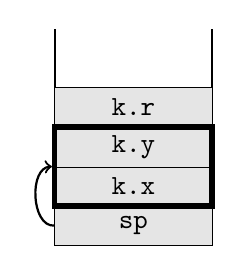
\begin{tikzpicture}
	\tikzstyle{Node} = [rectangle, minimum width=2cm, minimum height=5mm, text centered, draw=black, fill= gray!20]
	\tikzstyle{Sikidom} = [rectangle, minimum width=2cm, minimum height=10mm, text centered, draw=black, line width = 2pt]
	\tikzstyle{Kor} = [rectangle, minimum width=2cm, minimum height=15mm, text centered, draw=red, line width = 3pt]
	\tikzstyle{arrow} = [thick,->,>=stealth]
	
	\draw [thick, black] (0, 0) -- (2, 0);
	\draw [thick, black] (0, 0) -- (0, 2.75);
	\draw [thick, black] (2, 0) -- (2, 2.75);
	\node (s) [Node] at (1,0.25) {\texttt{sp}};
	\node (x) [Node] at (1,0.75) {\texttt{k.x}};
	\node (y) [Node] at (1,1.25) {\texttt{k.y}};
	\node (r) [Node] at (1,1.75) {\texttt{k.r}};
	\node (sikidom) [Sikidom] at (1,1) {};
	\path[every node/.style={font=\sffamily\small}]
	(s) edge[bend left = 90, thick, ->] node [right] {} (sikidom);
\end{tikzpicture}
\hspace{1cm}
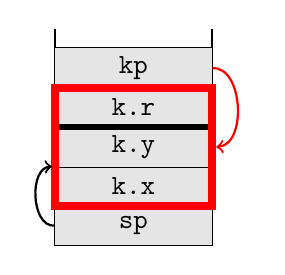
\begin{tikzpicture}
	\tikzstyle{Node} = [rectangle, minimum width=2cm, minimum height=5mm, text centered, draw=black, fill= gray!20]
	\tikzstyle{Sikidom} = [rectangle, minimum width=2cm, minimum height=10mm, text centered, draw=black, line width = 2pt]
	\tikzstyle{Kor} = [rectangle, minimum width=2cm, minimum height=15mm, text centered, draw=red, line width = 3pt]
	\tikzstyle{arrow} = [thick,->,>=stealth]
	
	\draw [thick, black] (3, 0) -- (5, 0);
	\draw [thick, black] (3, 0) -- (3, 2.75);
	\draw [thick, black] (5, 0) -- (5, 2.75);
	\node (s2) [Node] at (4,0.25) {\texttt{sp}};
	\node (x2) [Node] at (4,0.75) {\texttt{k.x}};
	\node (y2) [Node] at (4,1.25) {\texttt{k.y}};
	\node (r2) [Node] at (4,1.75) {\texttt{k.r}};
	\node (kp) [Node] at (4,2.25) {\texttt{kp}};
	\node (sikidom2) [Sikidom] at (4,1) {};
	\node (kor) [Kor] at (4,1.25) {};
	
	\path[every node/.style={font=\sffamily\small}]
	(s2) edge[bend left = 90, thick, ->] node [right] {} (sikidom2);
	\path[every node/.style={font=\sffamily\small}]
	(kp) edge[bend left = 90, thick, red, ->] node [right] {} (kor);
\end{tikzpicture}
		
		\caption{A \texttt{dynamic\_cast} működése.}\label{fig_dynamic_cast}
	\end{figure}
	Ez leginkább 3 dologra jó, leszármazott típusról bázis típusra konvertálásra (\textit{upcast}), bázisról leszármazottra (\textit{downcast}), valamint többszörös öröklődésnél bázisok közötti váltásra (\textit{sidecast}).
	
	A \texttt{dynamic\_cast} futási időben végzi a konverziót. Természetesen előfordulhat az, hogy a konverzió nem lehetséges:
	\begin{lstlisting}
Sikidom *s = new Sikidom;
Kor *k = dynamic_cast<Kor*>(*s);
	\end{lstlisting}
	Ebben az esetben egy hibás downcast-ot csináltunk, hisz \texttt{s}-nek a dinamikus típusa is \texttt{Sikidom}. Mivel minden \texttt{Kor} \textit{az egy} \texttt{Sikidom}, de ez fordítva nem igaz, így a konverzió nem lehetséges. Ilyenkor a \texttt{dynamic\_cast} nullpointert ad vissza. Ha referenciákkal jutunk ilyen helyzetbe, akkor egy \texttt{std::bad\_cast} típusú kivételt fog dobni.
	
	\smallskip
	Tekintsünk példát a \texttt{dynamic\_cast} működésére:
	\begin{lstlisting}
class Base 
{
	virtual ~Base(){} //polimorfizmus szükséges
};
class DerivedOne : virtual public Base {};
class DerivedTwo : virtual public Base {};
class DerivedLast : public DerivedOne, public DerivedTwo {};
//ez a jól ismert gyémántöröklés egy példája

int main()
{
	DerivedLast *dlp = new DerivedLast;
	Base *bp = dynamic_cast<Base*>(dlp); //upcast, dynamic_cast fölösleges
	DerivedOne *dop = dynamic_cast<DerivedOne*>(bp); //downcast
	DerivedTwo *dtp = dynamic_cast<DerivedTwo*>(dop); //sidecast
	delete dlp;
	
	bp = new Base;
	dop = dynamic_cast<DerivedOne*>(bp);  //dop nullpointer
	delete bp;
	
	Base b;
	try
	{
		DerivedOne &dor = dynamic_cast<DerivedOne&>(b); 
		//std::bad_cast-ot fog dobni
	}
	catch (std::bad_cast &exc)
	{
		std::cout << exc.what() << std::endl;
	}
}
	\end{lstlisting}
	
	Ez azonban nem hatékony, hisz a \texttt{dynamic\_cast} futási időben járja végig az öröklődési láncot. Ha nem vagyunk biztosak benne, hogy garantáltan lehetséges a castolás, akkor \texttt{dynamic\_cast}-ot érdemes használni, ha azonban biztosak vagyunk benne hogy az lehetséges, akkor \texttt{static\_cast} hatékonyabb.
	\subsection{static\_cast}
	Amennyiben teljesen biztosak vagyunk abban, hogy a cast szabályos, a \texttt{static\_cast} is használható mindenhol, ahol a \texttt{dynamic\_cast} is. Azonban ez az operátor nem végez semmilyen futási idejű ellenőrzést, így sikertelen kaszt esetén a kapott pointer/referencia invalid lesz (használata nem definiált viselkedést eredményez).
	
	\medskip
	A \texttt{static\_cast} fordítási időben konvertál egy típust egy másik típusra. Annak ellenére, hogy nem feltétlen biztonságos a használata polimorfikus osztályoknál, ez a konverzió végez ellenőrzéseket, méghozzá fordítási időben.
	\begin{lstlisting}
//a dynamic_cast-nál látott típusok itt is érvényesek
int main()
{
	Base *bp = new DerivedOne;
	DerivedOne *dop = static_cast<DerivedOne*>(bp); //ok
	DerivedLast *dlp = static_cast<DerivedLast*>(bp); //dlp invalid
	*dlp; //undefined behaviour
	
	int i = 5;
	double d = 5 / static_cast<double>(i);
	
	//malloc visszatérési típusa void*
	DerivedTwo *dtp = static_cast<DerivedTwo*>(malloc(sizeof(DerivedTwo)));
	free (dtp);
	
	Base ba[10];
	bp = static_cast<Base*>(ba);
}
	\end{lstlisting}
	E kettő kaszttal közel minden konverziót meg tudunk tenni, melyre szükségünk van és nem okoz nem definiált viselkedést.
	\subsection{const\_cast}
	A \texttt{const\_cast} az egyik a két veszélyesebb kaszt közül. Használata csak kivételes esetekben elfogadható, ugyanis nagyon sok galibát okozhat. 
	
	A \texttt{const\_cast} egy konstans objektumról ,,lekasztolja'' a konstansságot:
	\begin{lstlisting}
void print(int *param) { printf("%i", *param); }

int main()
{
	const int a = 0;
	print(const_cast<int*>(&a));
}
	\end{lstlisting}
	A fenti példa jól demonstrál egy tipikus helyzetet, amikor szabályos a \texttt{const\_cast} használata. Lévén C-ben nem létezett korábban a \texttt{const} kulcsszó, ezért mindent vagy érték szerint vagy nem konstans pointerrel vettek át. Ennek egyik következménye az, hogyha egy régi, C-s függvényt kell igénybe vennünk, mely nem módosítja a paramétert azonban nem konstansként várja, akkor le kell ,,szednünk'' a konstans objektumainkról a konstansságot.
	
	\smallskip
	Amennyiben egy nem konstans objektumra konstans referenciával vagy pointerrel hivatkozunk, abban az esetben a nem konstanssá castolt referencián vagy pointeren keresztüli módosítás legális. Amennyiben azonban egy adott objektum konstansként lett deklarálva, annak a módosítása nem definiált.
	\begin{lstlisting}
int main()
{
	int i = 3;
	const int& cref_i = i; 
	const_cast<int&>(cref_i) = 4; // ok, megváltoztatja i értékét
	
	const int j = 3;
	int* pj = const_cast<int*>(&j); // maga a cast legális
	*pj = 4; // a módosítás már undefined behaviour
}
	\end{lstlisting}
	\subsection{reinterpret\_cast}
	Mind közül a legveszélyesebb a \texttt{reinterpret\_cast}: két tetszőleges típus között végez konverziót, ha értelmezhető az, ha nem. Az értelmes konverziók közül egyetlen eset kivételével minden esetben a fenti 3 cast végre tudja hajtani a konverziót helyesen és sokkal biztonságosabban. Ez azt jelenti, hogy a \texttt{reinterpret\_cast} használata közel kivétel nélkül elkerülendő.
	
	\smallskip
	Az egyetlen konverzió, mely értelmes, és a fentiek nem képesek végrehajtani, amikor polimorfikus osztályoknál egy leszármazottat egy privát ősosztály típusra konvertálunk.
	\begin{lstlisting}
class MyVector : private std::vector<int> {};

MyVector *mvp = new MyVector;
std::vector<int> *vp = reinterpret_cast<std::vector<int>*>(mvp);
	\end{lstlisting}
	Azonban hiába szabályos ez a konverzió, rengeteg veszélyforrást tartalmaz, hisz a privát öröklés általában épp ennek a megakadályozására szolgál.
	\subsection{C-szerű cast}
	A C-szerű castok, vagy más néven \textit{C-style casts} olyan konverziók, melyek a fenti konverziókat próbálják meghívni, a \texttt{dynamic\_cast} kivételével. Amennyiben az egyik nem sikerül, a következőre haladnak. Ennek az értelemszerű hátránya az, hogy ha mind a \texttt{static\_cast}, mind a \texttt{const\_cast} sikertelen, akkor a \texttt{reinterpret\_cast}-ot fogja használni.
	\begin{lstlisting}
int main()
{
	float a = (float)10; //static_cast kerül meghívásra
	const int a;
	int &b = (int&)a; //const_cast
	Base *bp = (int*)b; //reinterpret_cast 
}
	\end{lstlisting}
	A \texttt{reinterpret\_cast}-tal ellentétben \textbf{soha} sincs szükség erre a cast-ra, csak a C-vel való kompatibilitás miatt része még a nyelvnek.
	\section{Implicit konverziók}
	%TODO ez most legyen elég, de azért lehet kéne ezen finomhangolni.
	Implicit konverzióról akkor beszélünk, ha egy adott típusú objektumnak egy másik típusú objektumot adunk értékül, és az egyik objektum a másik típusára konvertálódik anélkül, hogy mi ezt a konverziót külön (explicit módon, pl. cast-ok segítségével) ,,kértük'' volna.
	
	A nyelv egyik érdekessége, hogy lévén a \texttt{char} típusok tudnak számokat tárolni, így egy \texttt{char} objektum könnyedén át tud konvertálni \texttt{int} típusúra. Példaképp, az \texttt{'a' + 'b'} összeadásnál a karakterek összeadása nem definiált, azonban \texttt{int}-ek között igen, így a fordító implicit módon átkonvertálja azokat \texttt{int}-é.
	
	Amennyiben a fordító megpróbál egy műveletet elvégezni, de típushiba miatt ez meghiúsul, megpróbálja az objektumokat átkonvertálni, lehetőleg veszteségmentesen. A fordító először implicit konverzióval próbálkozik, aztán egy felhasználó által definiált konverzióval, majd ismét egy implicit konverzióval. Amennyiben ezek után sem megvalósítható a művelet típushiba miatt, fordítási hibát kapunk.
	\subsection{Aritmetikai konverziók}
	Meglepő módon, két \texttt{int} szám hányadosa C++ban nem lebegőpontos típussal fog rendelkezni, hanem szintúgy \texttt{int}-el. A primitív típusok között szigorú konverziós szabály van. Amennyiben például azt szeretnénk, hogy a 10/4 osztás végeredménye ne egész legyen, akkor az \texttt{/} operátor legalább egyik operandusának lebegőpontosnak kell lennie, pl. így: \texttt{10/4.0}
	
	Általános szabály az, hogy ha két típus eltér aritmetikai műveleteknél, akkor konvertálni kell, és mindig a kisebb méretű típust konvertáljuk a nagyobba.
	\begin{compactenum}
		\item Ha az egyik típusa \texttt{long double}, akkor a másikat is \texttt{long double}-ra konvertáljuk.
		\item Különben ha az egyik operandus \texttt{double}, akkor másik is \texttt{double} lesz.
		\item Különben, ha az egyik \texttt{float}, akkor a másik is \texttt{float} lesz.
		\item Amennyiben egyik operandus se lebegőpontos, akkor ha az egyik operandus \texttt{unsigned long}, akkor a másik is ez lesz.
		\item Ha az egyik operandus \texttt{long}, a másik pedig \texttt{unsigned int}, akkor előfordulhat az, hogy a két típus ugyanakkora tárterületen van tárolva (a primitív típusok méreteiről később lesz részletesekben szó). Ha az \texttt{int} és a \texttt{long} mérete megegyezik, akkor \texttt{unsigned
			long} lesz mindkét operandus. Különben ha a \texttt{long} nagyobb, akkor \texttt{long}-gá konvertálódik a másik.
		\item Különben ha az egyik \texttt{long}, a másik pedig NEM \texttt{unsigned int}, akkor \texttt{long}-gá konvertálódik a másik operandus.
		\item Különben, ha az egyik operandus \texttt{unsigned int}, a másik is kovnertálódik \texttt{unsigned int}-té.
		\item Különben minden \texttt{int}-té konvertálódik, ha egyik korábbi sem teljesült.
	\end{compactenum}
	\subsection{Logikai konverzió}
	Amikor \texttt{for} ciklusban vagy \texttt{if} ágban meg kell adnunk egy logikai értéket, akkor ott gyakran történhez implicit konverzió. Példaképp minden lebegőpontos vagy egész szám ami 0-tól különböző \texttt{true} értékre konvertálódik, míg 0 érték \texttt{false}-ra. Pointereknél minden nem nullpointer \texttt{true}.
	\subsection{Template-ek és az implicit konverzió}
	Template-eknél nem minden esetben megengedett az implicit konverzió. Tekintsük az alábbi kódot:
	\begin{lstlisting}
template <class T>
T max(T a, T b)
{
	return a < b ? b : a;
}

int main()
{
	std::cout << max(1, 1.5) << std::endl;
}
	\end{lstlisting}
	Hibaüzenetet kapunk, miszerint a template paraméter dedukció nem volt sikeres, hiszen \texttt{T}-nek vagy \texttt{int}-nek, vagy \texttt{double}-nak kéne lennie, de egyszerre nem tud az lenni.
\end{document}
